\documentclass[class=article, crop=false]{standalone}

\usepackage{graphicx}	% Including figure files
\usepackage{amsmath}	% Advanced maths commands
\usepackage{amssymb}

\newcommand{\fthin}{f_{\rm thin\,disk,\,recent}}
\newcommand{\tcools}{t_{10^5\,{\rm K}}}
\newcommand{\tacc}{t_{\rm acc}}
\newcommand{\Mdot}{\dot{M}}
\newcommand{\Rvir}{r_{\rm vir}}
\newcommand{\nH}{n_{\rm H}}
\newcommand{\Tvir}{T_{\rm vir}}
\newcommand{\msun}{{\rm M}_\odot}
\newcommand{\vvir}{v_{\rm vir}}
\newcommand{\Nsample}{17}
\newcommand{\Rcirc}[0]{r_{\rm circ}}
\newcommand{\vc}[0]{v_{\rm c}}
\newcommand{\mturb}[0]{\mathcal{M}_{\rm turb}}

\begin{document}

% HOT IN HALO
\begin{figure*}
    \centering
    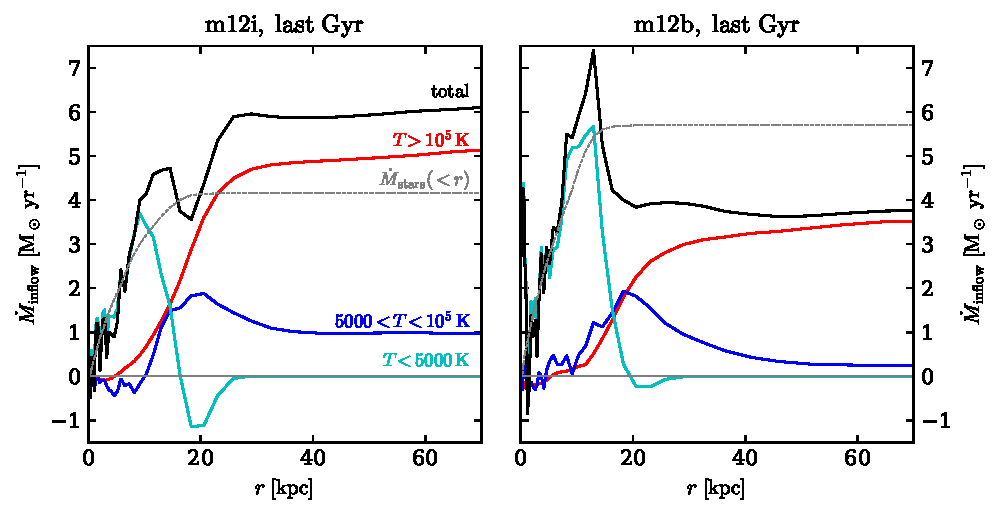
\includegraphics[width=\textwidth]{figures/Mdot.pdf}
    \caption{
    Average mass inflow rate versus gas temperature, during the last Gyr prior to $z=0$ in the same haloes as in Fig.~\ref{f: stars}.
    The galaxy radius $r_{\rm gal}=4 r_{\star,0.5}$ is marked in the panels. 
    Hot accretion ($T>10^5$ K) dominates the mass inflow onto thin-disk galaxies at $r \gtrsim r_{\rm gal} \sim 10-20$ kpc.
    Cold accretion ($T<10^5$ K) dominates the inflow onto the  
    % within the galaxy in thin disk galaxies, and 
    % in the halo of the lower-mass 
    irregular galaxy.
    }
    \label{f: Mdot}
\end{figure*}

In this appendix we analyze if inflow is dominated by hot or cold gas, which allows us to distinguish a hot inflow from the accretion of cool clouds (formed, e.g., via instabilities).
Fig.~\ref{f: Mdot} shows the mass inflow rate versus radius for hot gas (red curves; $T>10^5$ K) and for cool gas (blue curves; $T < 10^5\,{\rm K}$),  for the four simulations shown in Fig.~\ref{f: stars}. 
We calculate the mass inflow rate at a given radius as
\begin{equation}
     \Mdot(r) = \frac{\int_{\rm shell} v_r dm}{\Delta r} = \frac{M_{\rm shell}}{\Delta r} \langle v_r\rangle_{\rm mass\, weighted}
     \label{e: Mdot}
\end{equation}
where $\Delta r=0.05\,{\rm dex}$ is the shell thickness, and the integration is done on all particles with centers within the shell which satisfy the appropriate temperature cut. 

% Consequences
In the three MW-mass galaxies with a large thin disk fraction, at halo scales of $r>20$ kpc the inflow is dominated by hot gas, where in \texttt{m12i} and \texttt{m12b} $\Mdot$ of the hot gas is larger by a factor of $\gtrsim 4\times$ than that of cool gas.
The greater mass flux of hot gas indicates that the dominant form of accretion is an inflowing hot phase, rather than cold streams or cool clouds precipitating from the hot phase.
In contrast, in the lower mass galaxy shown in the bottom right the inflow is dominated by cool gas, while the hot gas is outflowing out to $\approx50$ kpc.
Fig.~\ref{f: Mdot} also shows that the inflow rate of hot gas in the MW-mass galaxies drops within $r_{\rm gal}$, reflecting the cooling of the hot inflow at the galaxy-halo interface, as shown in \S\ref{s: characteristics -- cools}.


\end{document}